% !TeX spellcheck = fr_FR
\chapter{Chapitre 1 : Analyse}

\section{Description du projet}
L'objectif principal de ce projet est d'exploiter le parallélisme offert par les \gls{fpga}, afin de calculer les fonctions de hachage nécessitant beaucoup de temps de calculs. 
Le but étant d'avoir au final un système plus efficient que les solutions actuelles sur \gls{gpu} et de la rendre la plus scalable possible.
Il est aussi nécessaire d'avoir une certaine communication entre le \gls{pc} de l'attaquant et le \gls{fpga}, afin que l'attaquant puisse fournir les informations nécessaires au cassage du mot de passe.

\begin{figure}[tbph!]
	\centering
	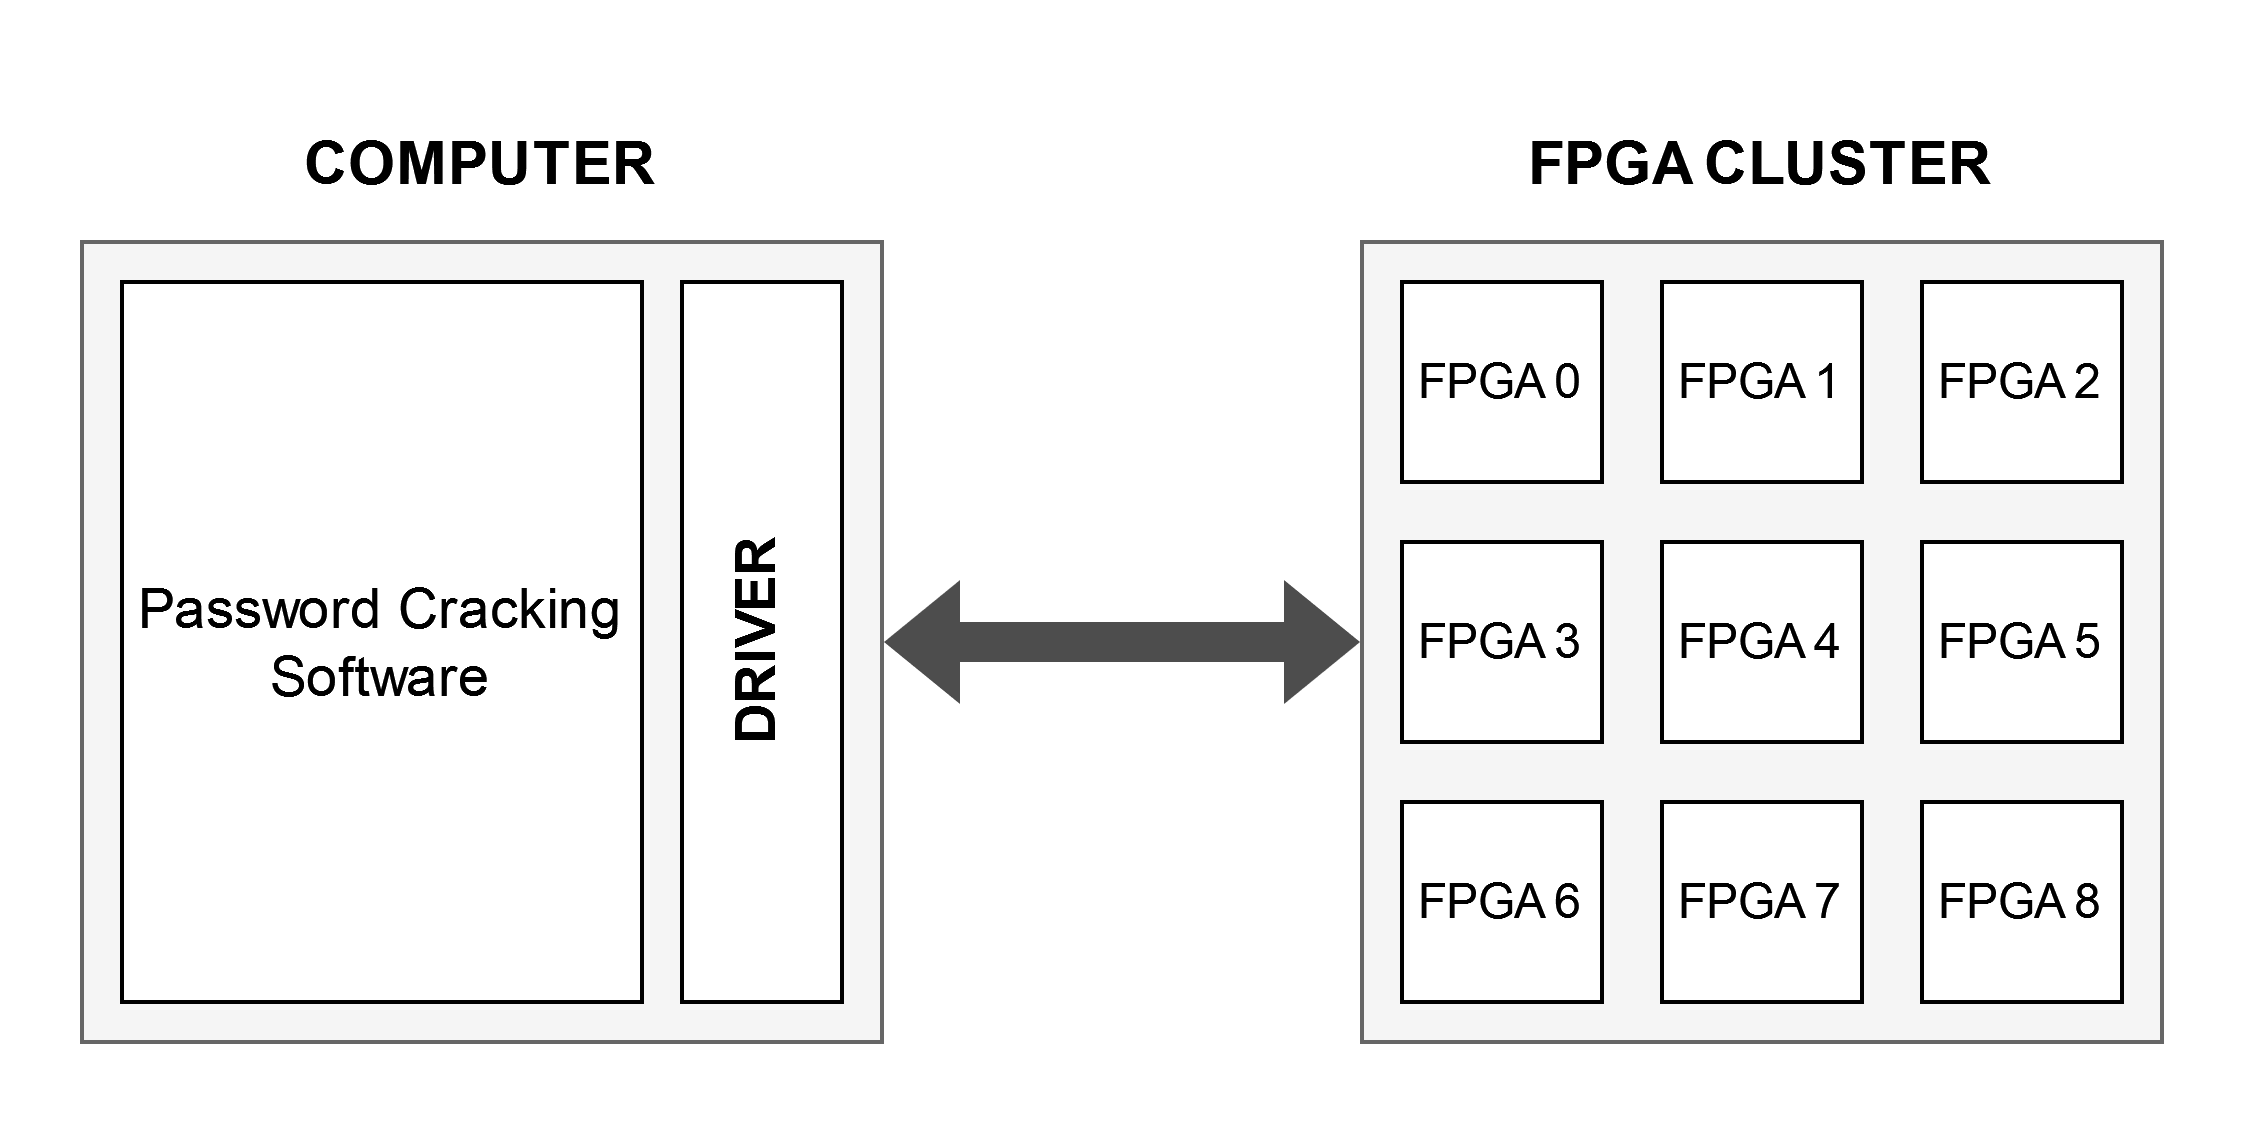
\includegraphics[width=0.9\linewidth]{objectif}
	\caption[Diagramme général]{Diagramme général. Source : réalisé par Kandiah Abivarman}
	\label{fig:objectif}
\end{figure}

L'idéal serait d'avoir deux solutions, une première qui consiste à simplifier le système en générant directement les mots de passe dans le \gls{fpga} à l'aide de système de compteur.
Puis la deuxième solution, serait de générer les mots de passe sur le \gls{pc} et d'ensuite les transférer au \gls{fpga} pour qu'il puisse faire les calculs.
La première solution sera plus simple à mettre en place, car ne nécessite pas de communication rapide entre le \gls{pc} et le \gls{fpga}
et la deuxième solution sera plus complexe à mettre en place, mais nous apportera une plus grande flexibilité au niveau de la génération de mots de passe, nous permettant notamment une attaque par dictionnaire\footcite{noauthor_attaque_2021}.

\section{Méthodes de communication}

Pour la communication entre le \gls{pc} et la carte \gls{fpga}, j'ai pu identifier trois méthodes :
\begin{enumerate}
	\item L'\gls{uart} qui est la méthode la plus simple à mettre en place
	\item Le \gls{pcie} qui est la méthode de communication la plus rapide
	\item Le Ethernet qui est la méthode la plus scalable.
\end{enumerate}

Dans ce projet, j'ai décidé de travailler avec l'\gls{uart} et le \gls{pcie}. 
Toutefois, même si je n'ai pas utilisé l'Ethernet durant ce projet, cette méthode reste intéressante pour une solution nécessitant un grand nombre de \gls{fpga}.

\subsection{UART}

L'\gls{uart} est une méthode de communication avec laquelle je suis déjà familier. Il est assez simple de le mettre en place côté \gls{pc}, notamment en Python.
Pour ce qui est de l'\gls{uart} côté \gls{fpga}, j'ai déjà en ma possession du code \gls{vhdl} qui nous a été donné durant nos cours qui me permet aisément d'en faire.
Cette méthode est idéale pour le premier système dont la génération des mots de passe est faite directement dans le \gls{fpga}.
En effet, la communication servira seulement à configurer le système au début de l'attaque puis recevoir le résultat lorsque le bon mot de passe a été trouvé.

\begin{figure}[tbph!]
	\centering
	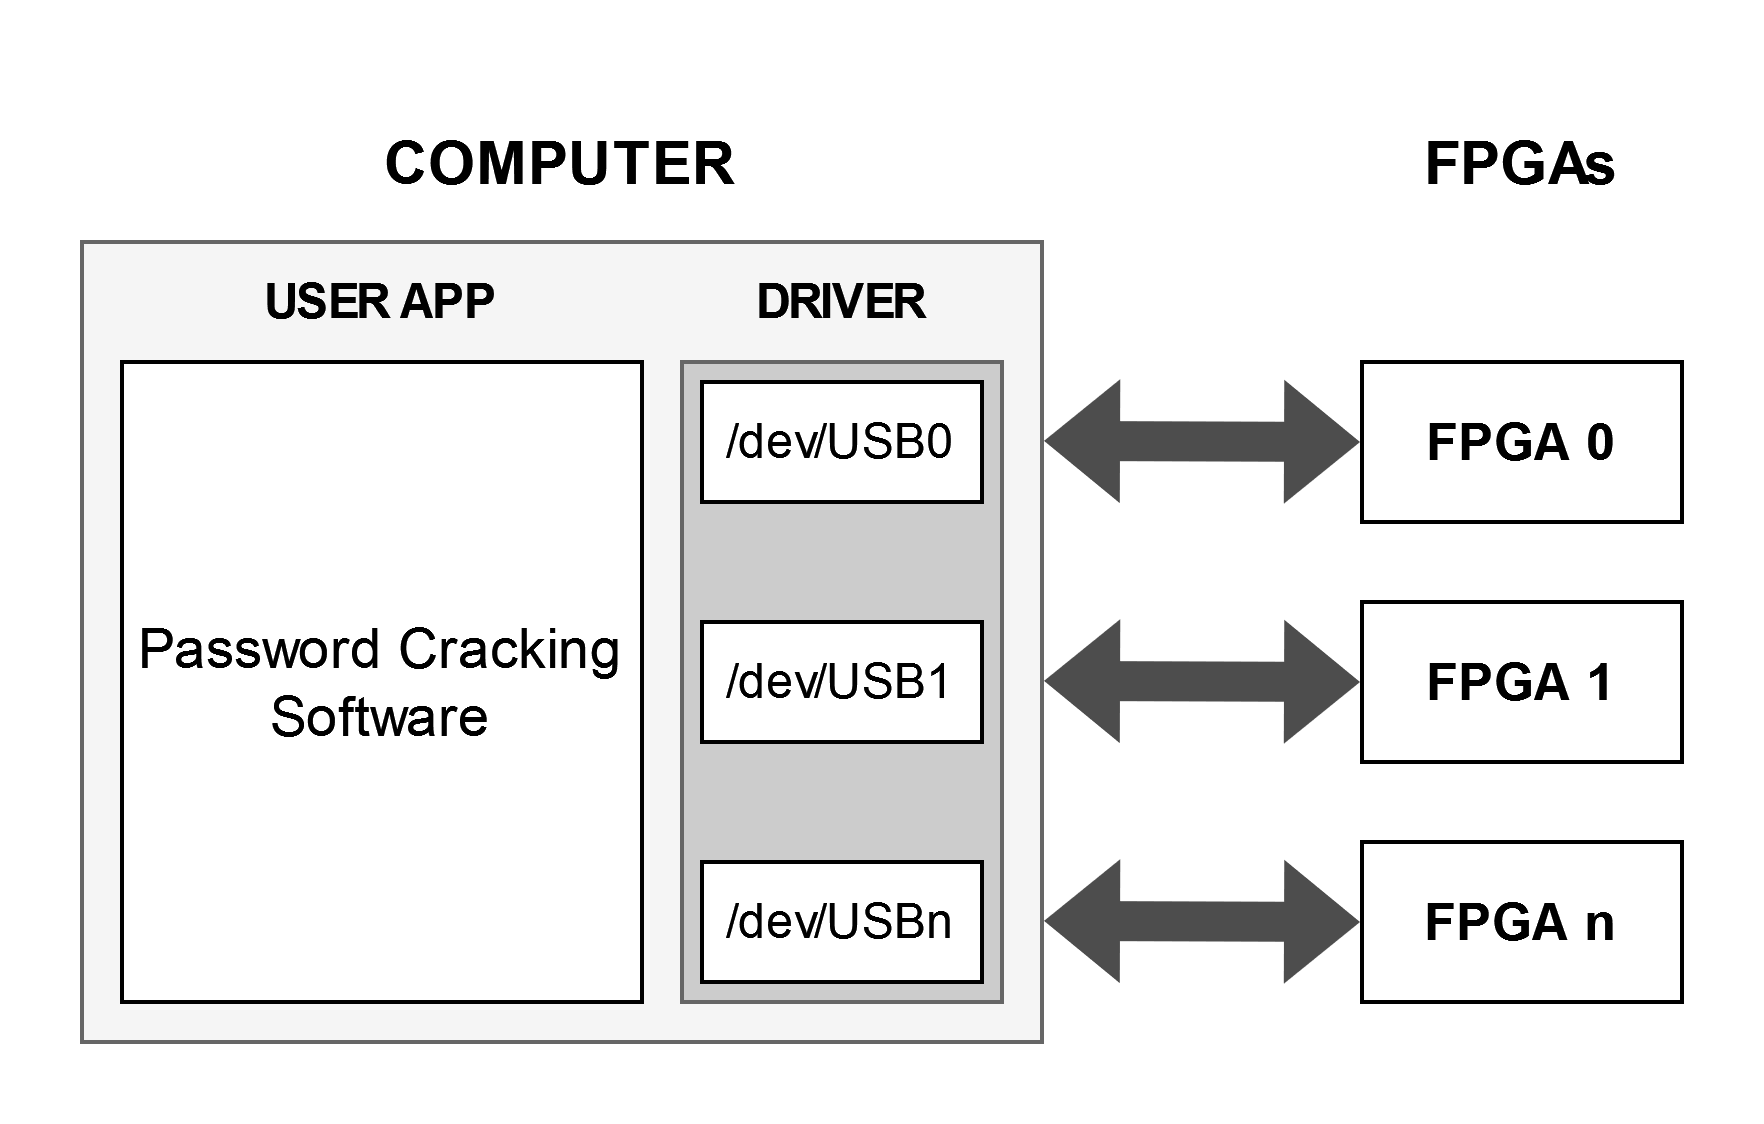
\includegraphics[width=0.8\linewidth]{general_uart}
	\caption[Diagramme général avec UART]{Diagramme général avec UART. Source : réalisé par Kandiah Abivarman}
	\label{fig:general_uart}
\end{figure}

Toutefois, afin d'avoir une communication robuste, il est nécessaire de mettre en place un système de paquet.
Le système de paquet devrait avoir un moyen de synchronisation et une vérification d'erreurs.


\subsection{PCIe}

Le \gls{pcie} est une méthode qui permet de transférer beaucoup de données à très haute vitesse.
Cette méthode de communication va être utilisé pour le deuxième système, celui-ci va nous permettre de transmettre les mots de passe depuis le \gls{pc} au \gls{fpga}.
En effet, il nous faut une communication rapide, car il faudrait pas que la communication soit le goulot d'étranglement de notre système.

Pour ce faire, du côté de l'\gls{fpga} il y a un bloc \gls{ip} qui est fourni qui permet d'interfacer avec le \gls{pcie}.
La difficulté provient majoritairement du \gls{pc}, car il va falloir mettre en place le driver \gls{pcie} nous-même.
Evidemment, il n'y a pas besoin de partir de zéro non plus, on peut retrouver des exemples de driver linux \gls{pcie} sur internet.

\begin{figure}[tbph!]
	\centering
	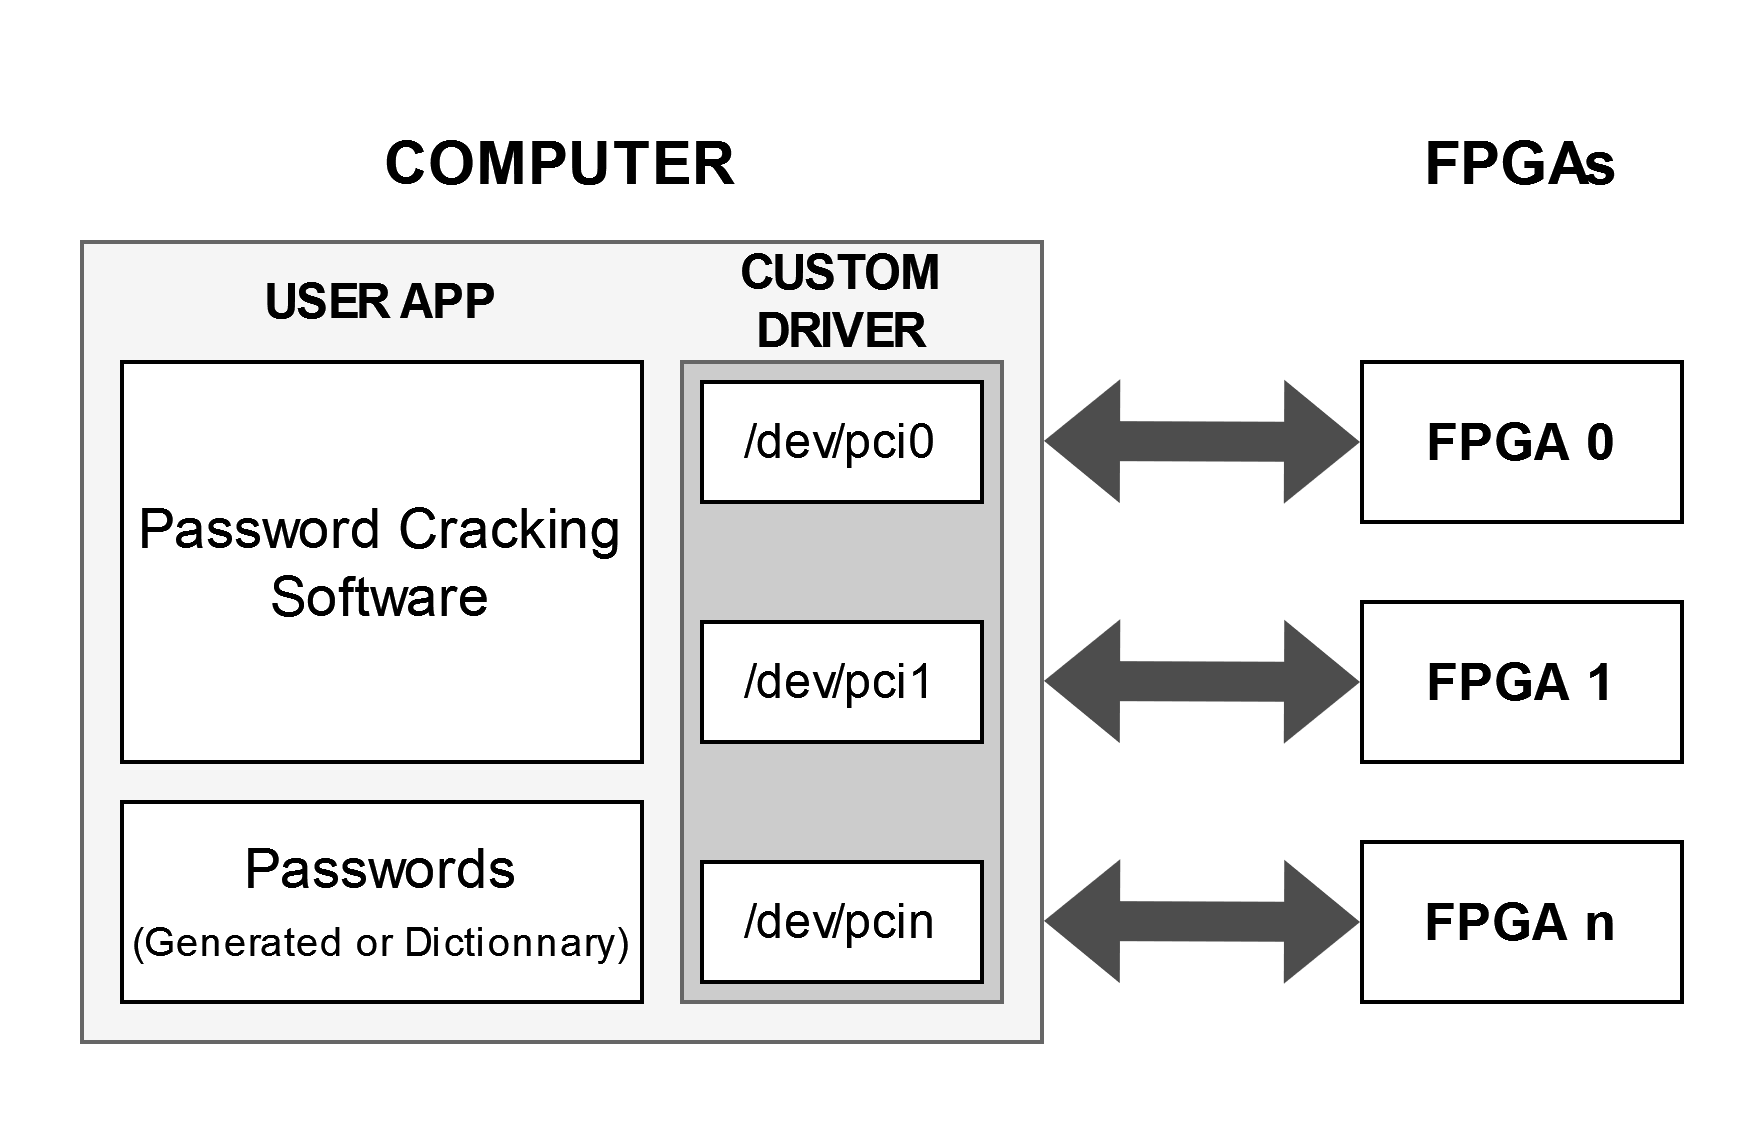
\includegraphics[width=0.8\linewidth]{general_pcie}
	\caption[Diagramme général avec PCIe]{Diagramme général avec PCIe. Source : réalisé par Kandiah Abivarman}
	\label{fig:general_pcie}
\end{figure}

\newpage

\section{Bcrypt}

Pour ce projet, nous avons décidé de cibler le Bcrypt, car c'est une fonction de hachage qui prend du temps à être calculé. 

Le Bcrypt est une fonction de hachage avec comme particularité, un paramètre supplémentaire qui est le cost (coût en français).
Ce paramètre va définir le nombre d'itérations que va prendre la fonction de hachage, de ce fait plus le cost est élevé, plus le calcul va prendre du temps.

\subsection{Algorithme}

L'algorithme du Bcrypt se base sur l'algorithme de chiffrement Blowfish\footcite{noauthor_blowfish_2019} qui est une fonction de chiffrement à clef symétrique, c'est-à-dire que la même clef est utilisée pour le chiffrement et le déchiffrement. 
L'algorithme du Bcrypt peut être divisé en deux grandes étapes.

On a une première étape qui est une phase de mise en place des clés symétriques. 
Dans cette étape, on va créer les clés de chiffrements à partir des paramètres d'entrée de la fonction de hachage (mot de passe, salt, cost). 
Cette première étape est la partie la plus coûteuse de la fonction, car la mise en place de la clé va prendre plus ou moins de temps en fonction du cost. 
Les clés de chiffrement sont composées de Subkeys qui est un tableau de 18 entiers de 32 bits et quatre \gls{sbox} qui sont chacun des tableaux de 256 entiers de 32 bits. 
Avant de calculer ces clés de chiffrements, ils sont tout d'abord initialisés avec les décimales de PI.

Puis il y a la deuxième étape, où l'on va utiliser les clés de chiffrement qui ont été calculées plus tôt afin de chiffrer la phrase magique "OrpheanBeholderScryDoubt", le chiffrement va être fait 64 fois.

\begin{figure}[tbph!]
	\centering
	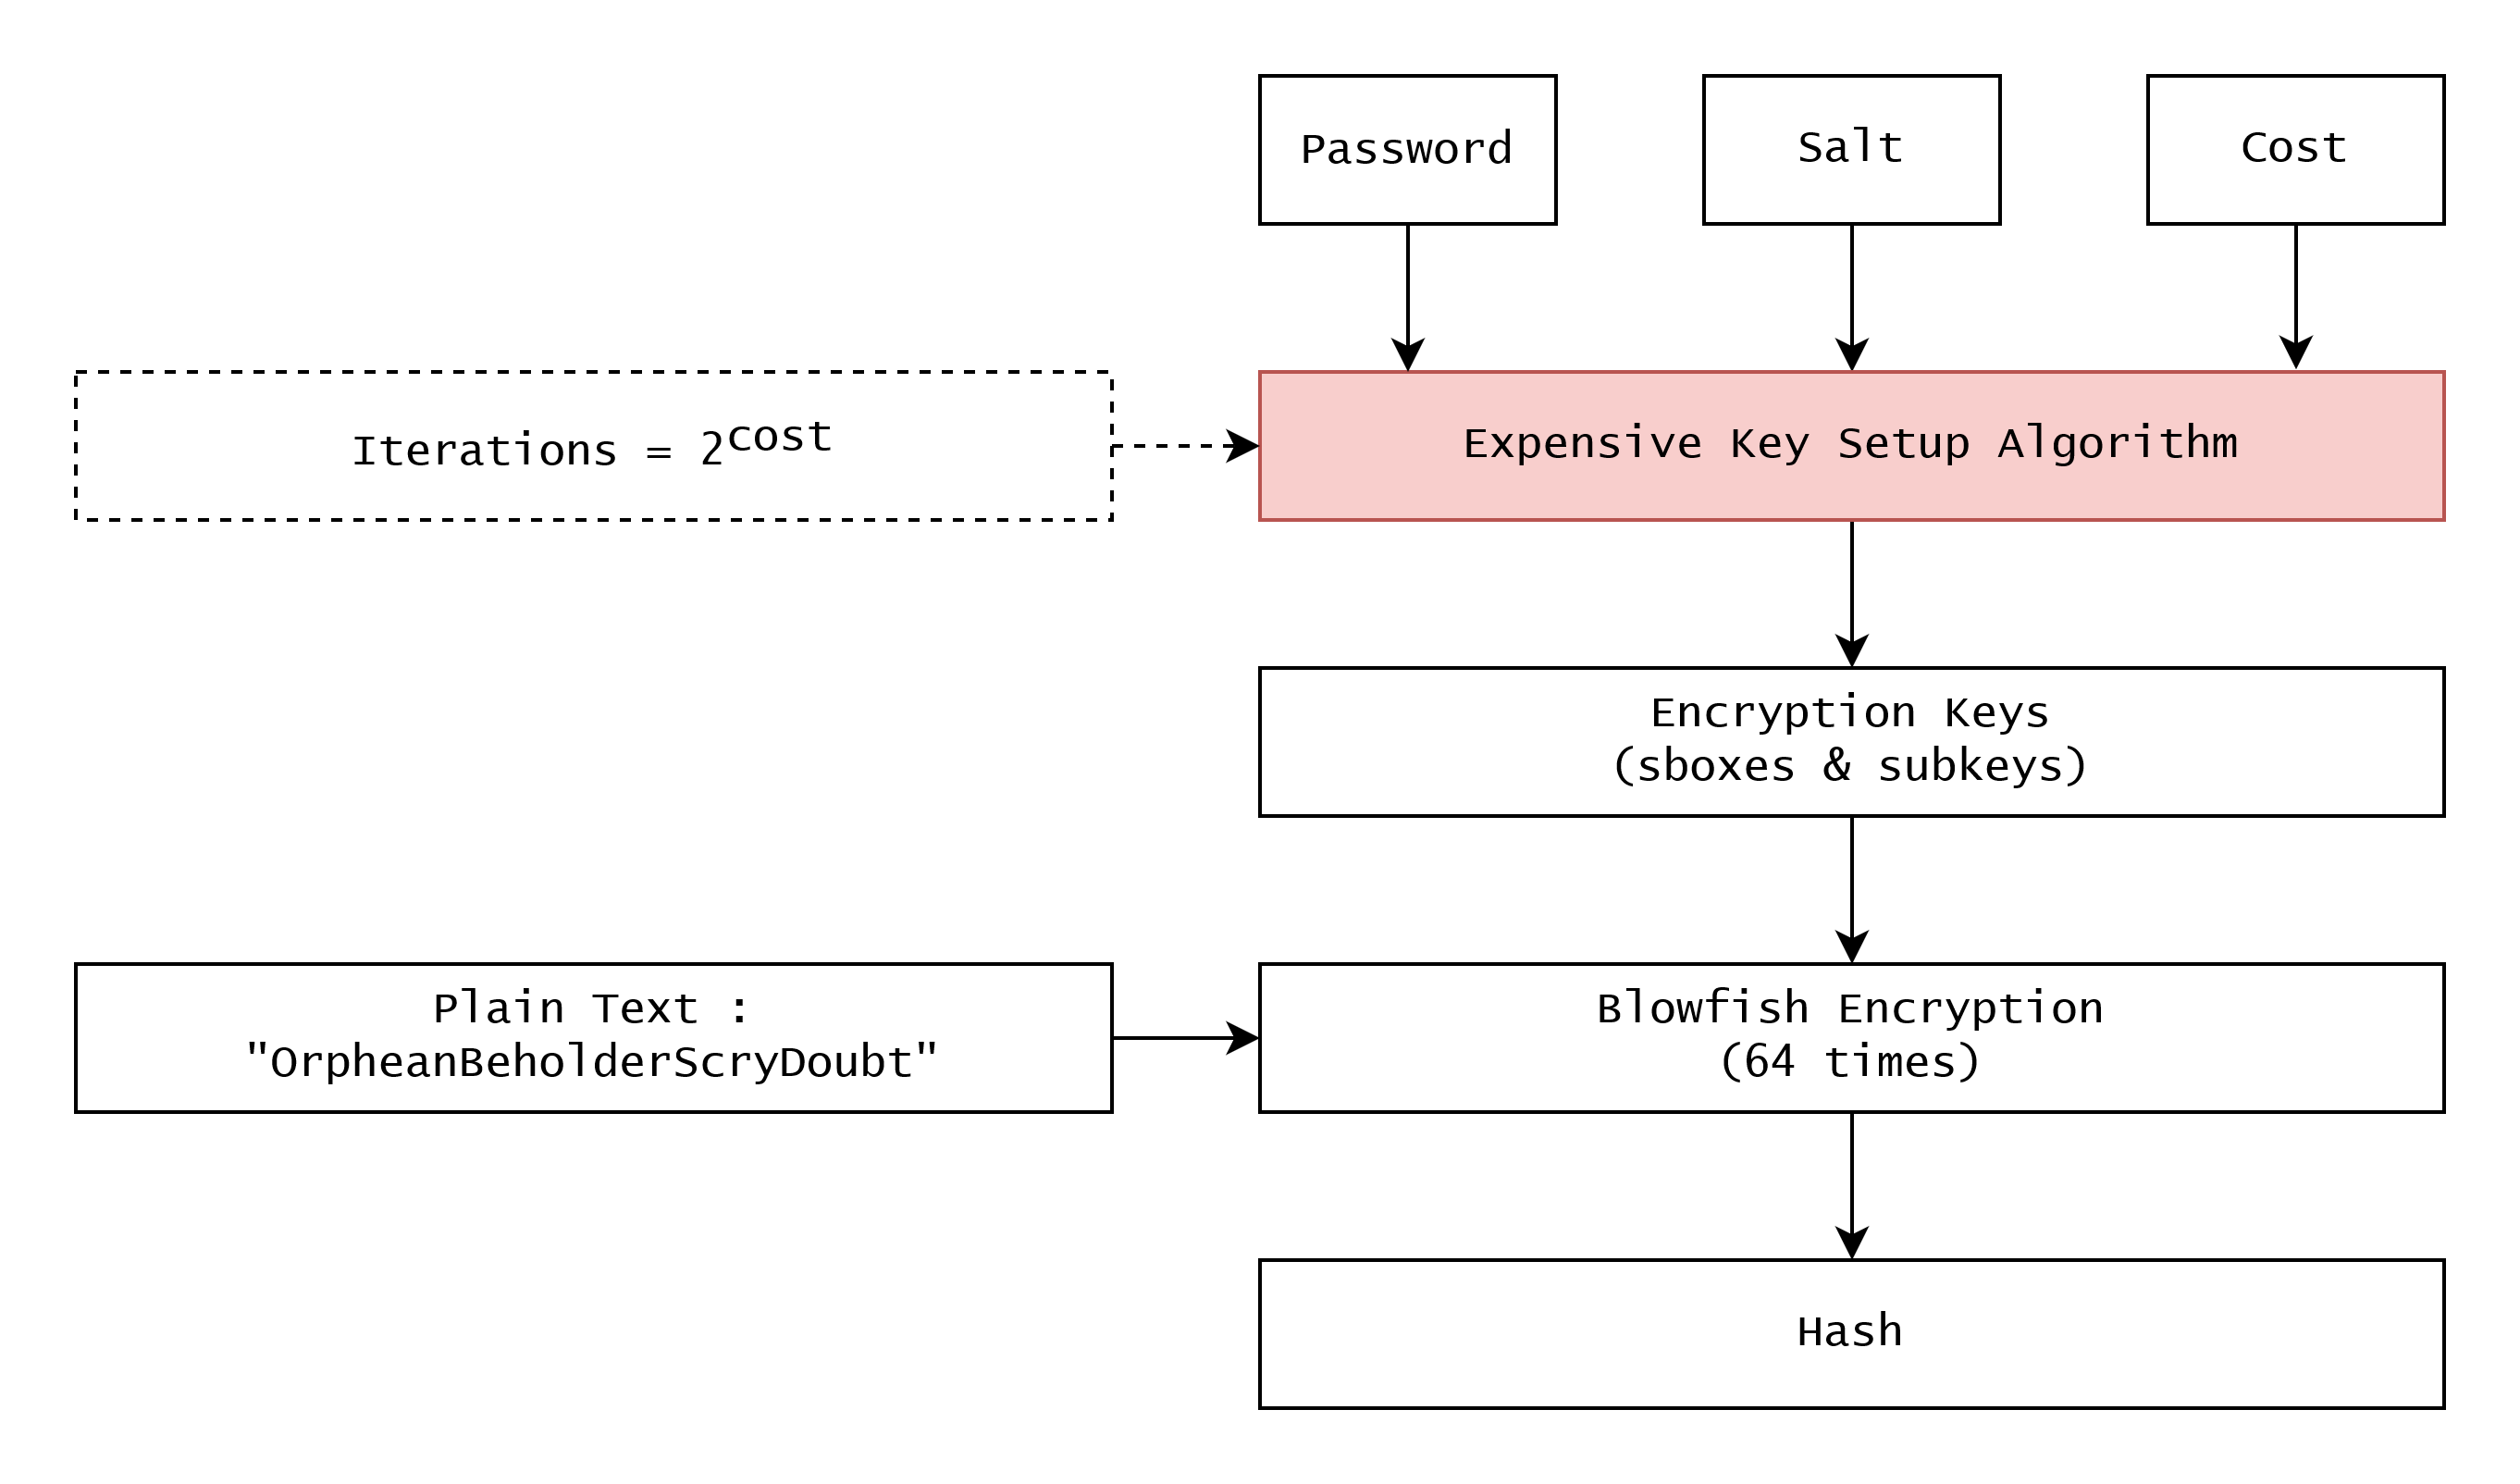
\includegraphics[width=0.7\linewidth]{bcrypt_algo}
	\caption[Algorithme Bcrypt]{Algorithme Bcrypt. Source : réalisé par Kandiah Abivarman}
	\label{fig:bcrypt_algo}
\end{figure}

\newpage

\subsection{Format du Hash}

Le hash généré par la fonction Bcrypt est généralement stocker sous une forme particulière. 

\begin{figure}[tbph!]
	\centering
	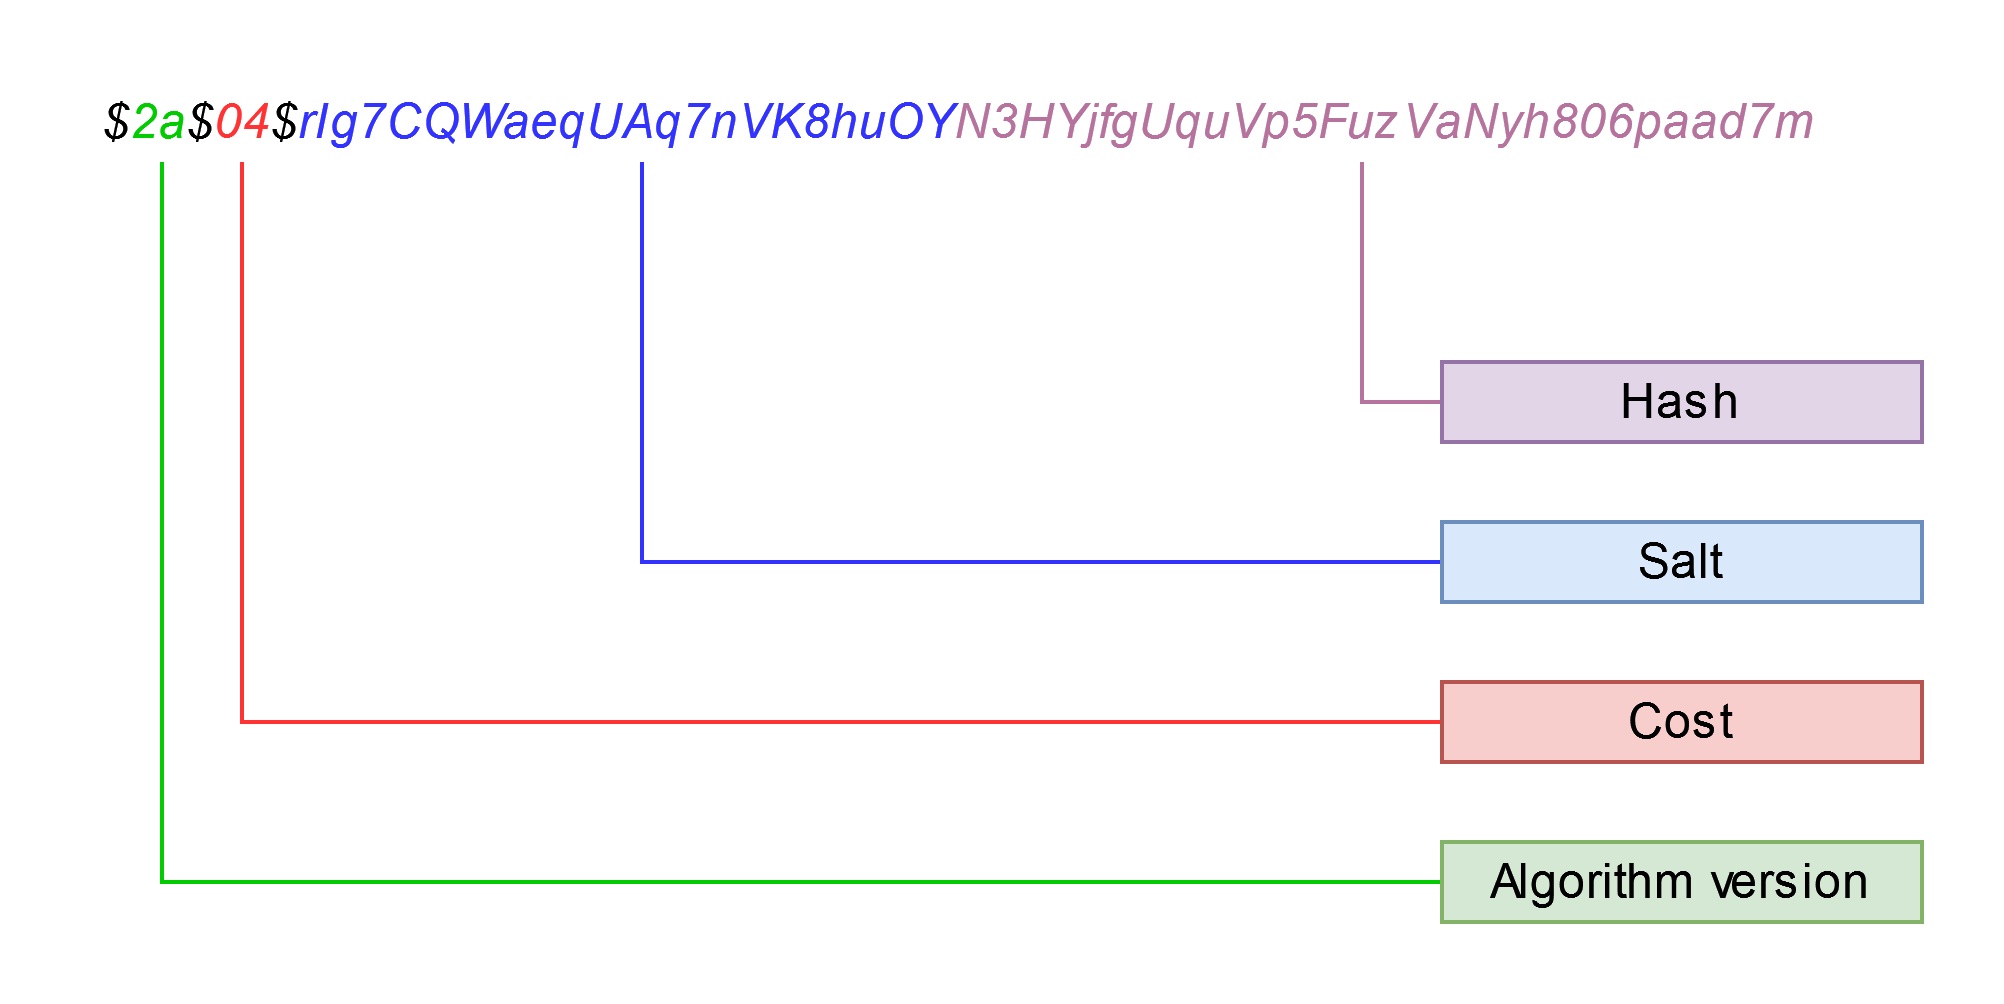
\includegraphics[width=0.7\linewidth]{bcrypt_hash_format}
	\caption[Format du hash Bcrypt]{Format du hash Bcrypt. Source : réalisé par Kandiah Abivarman}
	\label{fig:bcrypt_hash_format}
\end{figure}

On va avoir un premier champ qui contient la version de l'algorithme, un deuxième qui contient le cost de la fonction, un troisième avec le salt et le quatrième avec le hash généré. 
Le salt et le hash sont en base 64, mais il faut faire attention, car c'est une base 64 différente de la norme RFC 4648\footcite{josefsson_base16_2006} qui est couramment utilisé.

\begin{figure}[tbph!]
	\centering
	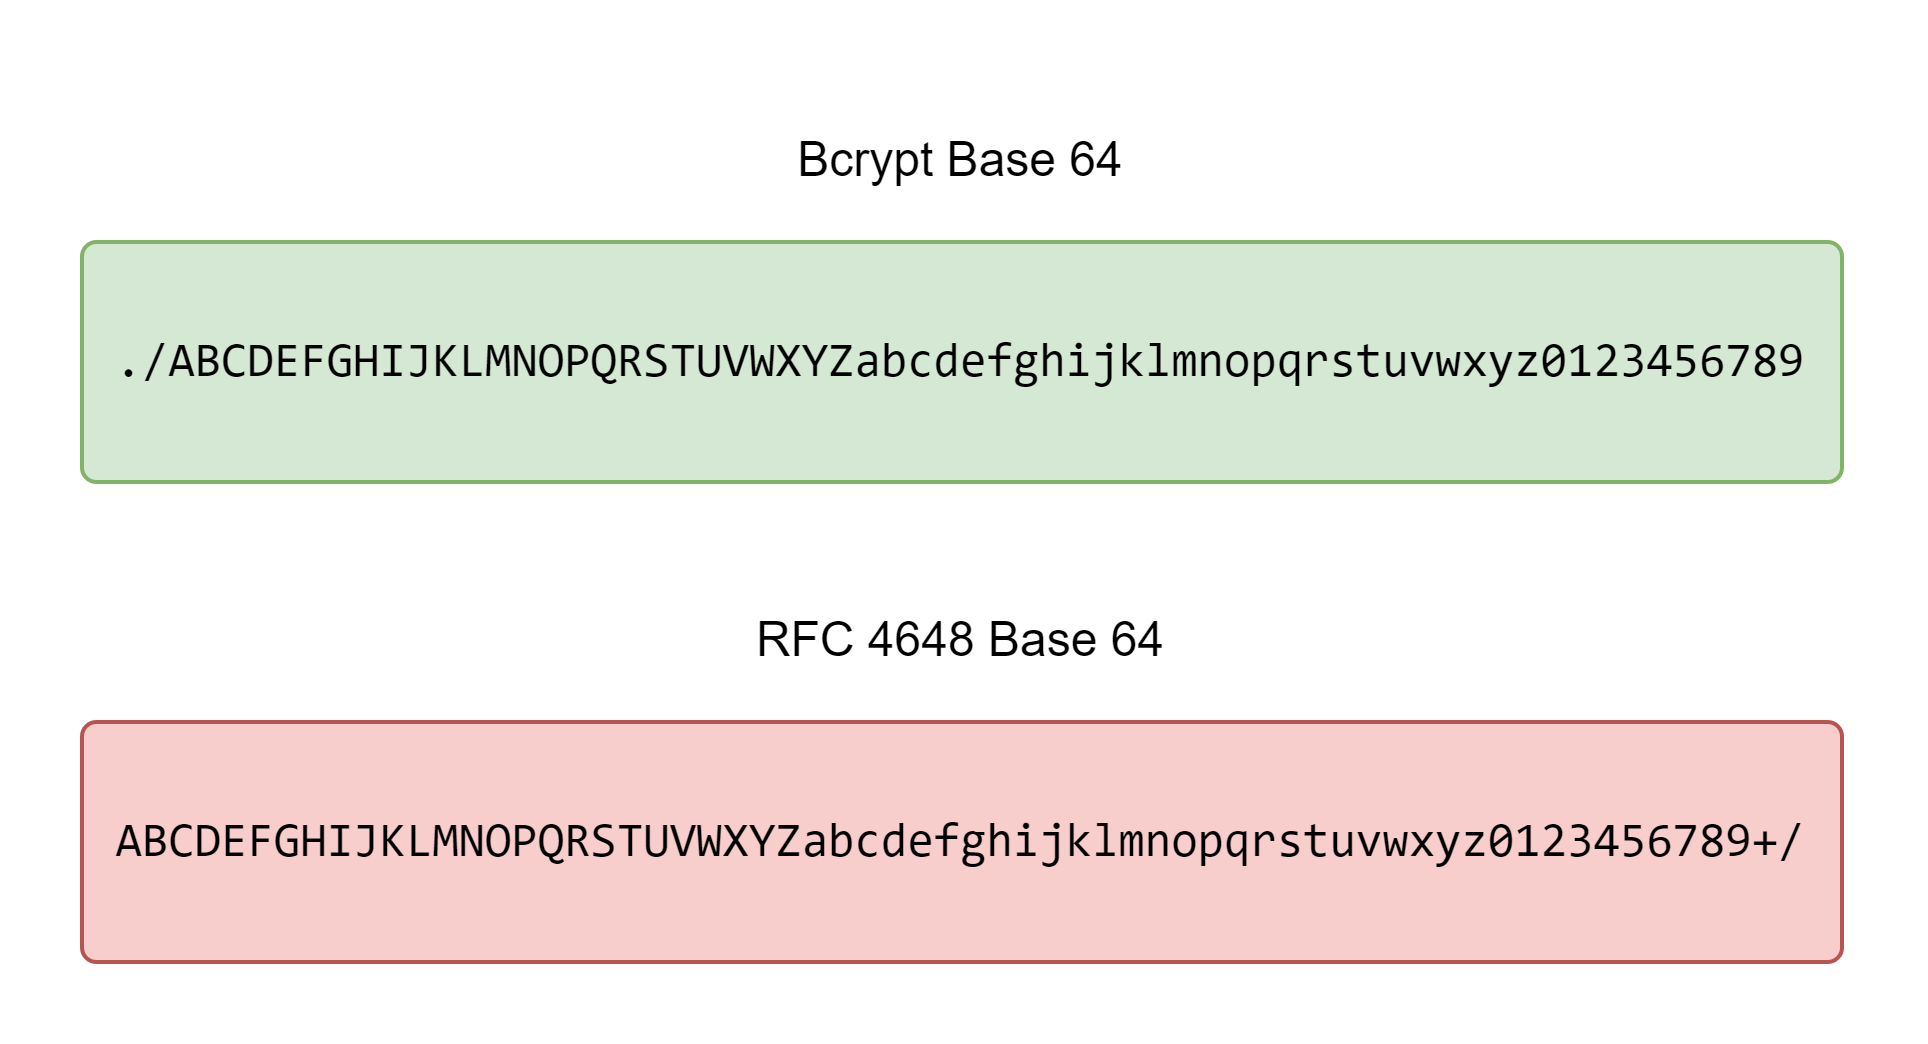
\includegraphics[width=0.7\linewidth]{base_64}
	\caption[Différence Base 64]{Différence Base 64. Source : réalisé par Kandiah Abivarman}
	\label{fig:base_64}
\end{figure}

\subsection{Implémentations Existantes}

Afin d'éviter de réinventer la roue, la première tâche que j'ai entrepris est de chercher afin de voir s'il n'existe pas déjà des implémentations existantes sur \gls{fpga}. 

D'après mes recherches, j'ai retrouvé seulement deux implémentations du Bcrypt sur FPGA. 
La première se situe dans le répertoire github de JohnTheRipper\footcite{noauthor_openwalljohn_2024} qui est un logiciel de cyber-sécurité destiné au craquage de mot de passe, l'implémentation a été faite en Verilog et spécifiquement pour la Ztex 1.15y qui est une carte FPGA assez ancienne et difficilement retrouvable. 
La deuxième est une implémentation faite en \gls{vhdl} que j'ai aussi retrouvé dans un répertoire github\footcite{noauthor_rub-hgihigh-speed_bcrypt_nodate}, accompagné d'un papier\footcite{wiemer_high-speed_2014} décrivant un travail de recherche effectué sur l'attaque de mot de passe sur FPGA. 
Pour ma part, connaissant seulement le \gls{vhdl} et ne comprenant pas réellement la structure de code du premier et par manque d'informations, j'ai préféré reprendre le code du deuxième. 

Le papier a été très instructif, j'ai pu notamment comprendre les différents choix qui ont été pris dans le code source. 
Malheureusement, tout n'a pas été documenté et le répertoire n'a pas été mis en place correctement. 
En effet, certains partie du code contenait des erreurs, les fichiers de tests étaient incomplets et des fichiers source semble avoir été retravaillé en aval.